\chapter{Sequence and Series}
I normally like to start this chapter with a very well known story. Let's go to a classroom in somewhere near 1785. The math teacher is a man who is not interested in teaching and wants to chat with the female school workers. So he decides that he must keep you all engaged and quiet while he tries to get a life partner. He writes on the board: $1+2+3+\dots +100$ Do not speak until complete\\
Saying that he leaves. While everyone else is diligently adding, one of the kid stands up after a minute and walks outside the class to find the teacher. "The answer is $5050$" he announces.\\
"It's wrong!" The teacher replies, as he doesn't really know the correct answer. He just figures that a 8 year old couldn't add this quickly.\\
The child replies, "Sir, its correct."\\
"Are you the teacher or am I?"\\
"With all due respect, sir it's correct."\\
"See, you could by no means add so quickly. You are just guessing."\\
"Sir, I didn't add much. I multiplied."\\
"What?"\\
"$1+100=101$, $2+99=101$ and so on, $50+51=101$. We have $50$ such pairs. So the answer must be $50*101=5050$."
The teacher patted the child, impressed. "Well that's something."\\
The child was the great mathematician Carl Friedrich Gauss. The teacher, although more intrested in love than math, took notice of Gauss's talents and worked actively with the university to nurture him.\\
\section{Some notes on notation}
\begin{definition}
    A sequence is an ordered list of numbers. A series is the sum of that list.
\end{definition}
This chapter will also be the first time we'll use the summation notation. Why use it instead of just some terms, $\dots$ and more terms? Here is a quote from Calculus II for Dummies.
\begin{quote}
    Mathematicians just love sigma notation for two reasons. First, it provides a convenient way to express a long or even infinite series. But even more important, it looks really cool and scary, which frightens non-mathematicians into revering mathematicians and paying them more money.
\end{quote}
\begin{definition}
    In the summation notation or sigma notation:\\
    \[\sum^b_{a=1}f(a)=f(1)+f(2)+\dots +f(b-1)+f(b)\]
\end{definition}
By the definition itself, we can state two very useful properties of sigma notation.
\begin{theorem}
Distributively
    \[\sum kf(x)=f\sum f(x)\]\\
Commutativity
    \[\sum[f(x)+g(x)]=\sum f(x) + \sum g(x)\]
\end{theorem}
And that's all I wish to tell you about notation. Let's come back to math now.
\section{Arithmetic Progression}
An arithmetic progression is the more a sequence of numbers such that the difference between any two consecutive terms is constant. This constant is called the common difference of the sequence. $8,11,14,17$ is an AP\\
More formally: \\
\begin{definition}
    The sequence $a_1, a_2, \ldots , a_n$ is an arithmetic progression if and only if $a_2 - a_1 = a_3 - a_2 = \cdots = a_n - a_{n-1}$
\end{definition}
Now Lets consider $a_1, a_2, a_3 \dots a_n$ an AP with common difference $d$.
\begin{theorem}
    The $n^{th}$ theorem of an Arithmetic Sequence is:\\
    \[a_{n}=a+(n-1)d\]
\end{theorem}
This follows from the definition. 
\begin{theorem}
    Number of terms in an AP:\\
    \[n=\frac{a_n-a_1}{2}+2\]
\end{theorem}
This follows from the $n^{th}$ term formula.
\begin{theorem}
    Average of n terms of AP:\\
    \[\frac{a_1+a_n}{2}\]
\end{theorem}
This also follows from the definition of AP.
\begin{theorem}
    Sum of n terms of an AP:
    \[\frac{a_1+a_n}{2}\cdot n\]\\
    \[=\frac{a_1+a_1+(n-1)d}{2}\cdot n\]\\
    \[=\frac{2a_1+(n-1)d}{2}\cdot n\]
\end{theorem}
This follows from the definition of average.\\
With these trivial observations in your toolkit, you can now make some remarkable observations.\\
Let's consider the AP $1,2,3,\dots,n$ with $a_1=1$ and $d=1$. Then\\
\begin{theorem}
     \[\sum^n_{k=1}k=\frac{n+1}{2}\cdot n=\frac{n(n+1)}{2}\]
\end{theorem}
The numbers which can be written in the form of $\frac{n(n+1)}{2}$ are called trianguler numbers. This is because a given thoose number of balls, we can arrange them into a perfect triangle with a base of $n$. \\
The theorem above can also be shown without words 
\begin{figure}
    \centering
    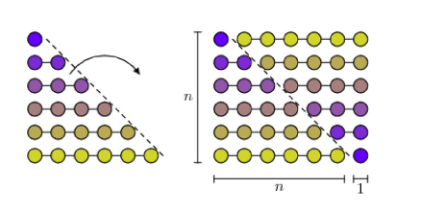
\includegraphics[width=0.5\linewidth]{Photos/triangle numbers.png}
    \caption{A proof without words for triangle numbers}
\end{figure}
You can also realize that this is exactly what Gauss did.
Now let's consider the AP $2,4,8,16 \dots 2n$
\begin{theorem}
    \[\sum^n_{k=1}2k=2\sum^n_{k=1}k=2*\frac{n(n+1)}{2}=n(n+1)\]
\end{theorem}
And finally, we'll consider the AP $1,3,5,7 \dots 2n-1$. It's sum is quite beautiful:\\
\begin{theorem}
    \[\sum^n_{k=1}2k-1=\sum^n_{k=1}2k-\sum^n_{k=1}1=n(n+1)-n=n(n+1-1)=n^2\]
\end{theorem}
This can also be basically proven without words as:\\
\begin{figure}
    \centering
    
\includegraphics[width=0.5\linewidth]{Photos/Sum of odds.png}
    \caption{Counting the number of squares in the alternating black and white gives us the proof}
    
\end{figure}
Now using whatever we just learnt, let's obliterate some questions.\\
\begin{example}
    (AIME 2012) The terms of an arithmetic sequence add to $715$. The first term of the sequence is increased by $1$, the second term is increased by $3$, the third term is increased by $5$, and in general, the $k$th term is increased by the $k$th odd positive integer. The terms of the new sequence add to $836$. Find the sum of the first, last, and middle terms of the original sequence.
\end{example}
\begin{proof}
    [Solution]
    Let's first realize that the question is asking the sum of first, last and the middle term of the AP. We also know that the middle term is the average of first and last term. So basically, we are looking for three times the middle term.\\
    Now let's find it. Let the sequence of $a_1,a_2,a_3 \dots a_n$:\\
    $\sum^n_{i=1}a_i=715$
    and adding the odd numbers\\
    $sum^n_{i=1}a_i+2n-1=835\\
    \iff sum^n_{i=1}a_i+sum^n_{i=1}2n-1=835\\
    \iff 715+n^2=835\\
    \iff n=11$\\
    Hence, we have $11$ terms in the sequence. As the sum is $715$, the middle term(or the average) is $65$. Hence, our answer is $65*3=195$\\
\end{proof}
\begin{example}
    (AIME 2005, edited)For each positive integer $k$, let $S_k$ denote the increasing arithmetic sequence of integers whose first term is $1$ and whose common difference is $k$. For example, $S_3$ is the sequence $1,4,7,10,\ldots.$ For how many values of $k$ does $S_k$ contain the term $2023$?
\end{example}
\section{Geometric Progression}
A lot of math jokes begin with: An infinite amount of mathematicians walk into a bar.\\
This can have one continuation for every mathematician in the bar. The most classic one is: The first one asks for a beer. The second one asks for half a beer. The third one asks for a quarter of a beer. The fourth one asks for an eighth of a beer... . The bartender pours two beers, saying "You guys ought to know your limits".\\
Let's try to understand what just happened. A geometric progression, is a sequence of numbers such that the ratio between any two consecutive terms is constant. This constant is called the common ratio of the sequence. For example, $1, 2, 4, 8$ is a geometric sequence with common ratio $2$ and $100, -50, 25, -25/2$ is a geometric sequence with common ratio $-1/2$; however, $1, 3, 9, -27$ and $-3, 1, 5, 9, \ldots$ are not geometric sequences, as the ratio between consecutive terms varies.
More formally, \\
\begin{definition}
    The sequence $a_1, a_2, \ldots , a_n$ is a geometric progression if and only if $a_2 / a_1 = a_3 / a_2 = \cdots = a_n / a_{n-1}$
\end{definition}
Let $g_1, g_2, g_3 \dots g_n$ be a GP with common ratio $r$.\\
\begin{theorem}
    The $n^{th}$ term in a GP is:
    \[g_n=g_1\cdot r^{n-1} \]
    \[g_n=g_m\cdot r^{n-m} \]    
\end{theorem}
This follows from the definition.
\begin{theorem}
    Sum of first n terms of a GP is:\\
    \[g_1\cdot \frac{r^n-1}{r-1}\]\\
    \textbf{NOTE: $\frac{r^n-1}{r-1}$ may be replaced with $\frac{1-r^n}{1-r}$ whenever convenient.}
\end{theorem}
\begin{proof}
This is one of the most beautiful proof in all of mathematics.
Let $S_n = a_1 + a_2 + \dots + a_n$\\
This can be re-written as:
$S_n = a_1 + a_1r + \dots + a_1r^{n-1}$
Multiplying both sides by $r$,
$S_nr = a_1r + a_1r^2 + \dots + a_1r^n$
Subtracting the original equation from this equation,\\
$S_nr - S_n = a_1r^n - a_1\\
\iff S_n(r-1)=a_1(r^n-1)\\
\iff S_n=\frac{a_1(r^n-1)}{r-1}$
\end{proof}
Quite cool, but here is something even more cool.
\begin{theorem}
    Sum of infinite terms of a converging GP:\\
    \[\frac{g_1}{1-r}\]\\
    \textbf{NOTE: This only holds for $-1\geq r \geq 1$, as other series sum keeps increasing to either $\infty$ or $-\infty$}
\end{theorem}
\begin{proof}
The proof is quite similar to above. With the only difference being that $n \rightarrow \infty$
Let $S_n = a_1 + a_2 + \dots$\\
This can be re-written as:
$S_n = a_1 + a_1r + \dots$
Multiplying both sides by $r$,
$S_nr = a_1r + a_1r^2 + \dots $
Subtracting this equation from the original equation,\\
$S_n-S_nr = a_1\\
\iff S_n(1-r)=a_1\\
\iff S_n=\frac{a_1}{1-r}$
\end{proof}
Now we can truly understand the joke at the start of the chapter.\\
The first mathematician asked for 1 beer, The second for half, the third for a qurter. This is a GP with $a=1$ and common ration $r=\frac{1}{2}$. So we can easily add it using the above formula:\\
$\frac{1}{1-\frac{1}{2}}=\frac{1}{\frac{1}{2}}=2$\\
Now let's blast some questions:\\
\begin{example}
    (AIME 2002) Two distinct, real, infinite geometric series each have a sum of $1$ and have the same second term. The third term of one of the series is $1/8$, and the second term of both series can be written in the form $\frac{\sqrt{m}-n}p$, where $m$, $n$, and $p$ are positive integers and $m$ is not divisible by the square of any prime. Find $100m+10n+p$.
\end{example}
\begin{proof}
    [Solution]
    Let the second term of both the series be $x$. Then the first term of the first series is $8x^2$ and the common ratio $\frac{1}{8x}$. As it's infinite sum is $1$,\\
    $1=\frac{8x^2}{1-\frac{1}{8x}}\\
    \iff 64x^3-8x+1=0\\
    \iff (4x-1)(16x^2+4x-1)=0
    \iff x=\frac{1}{4}, \frac{\sqrt{5}-1}{8}, \frac{-\sqrt{5}-1}{8}$\\
    As $x$ is of the form $\frac{\sqrt{m}-n}p$\\
    $\therefore x=\frac{\sqrt{5}-1}{8}\\
    \therefore m=5, n=1, p=8$\\
    Hence, $100m+10n+p=518$\\
\end{proof}
\begin{example}
    The sum of the first $2011$ terms of a geometric sequence is $200$. The sum of the first $4022$ terms is $380$. Find
the sum of the first $6033$ terms.
\end{example}
\section{Induction and Summation}
While many of the summations are quite trivial to derive, some of them cannot be derived. Only proven. These are typically observed and then proved using a technique called induction.\\
Almost everyone has once had fun arranging dominoes(or jenga bricks) in a row and starting a wave. Push the first domino and it topples the second, the second will topple the third and so forth until all the dominoes are toppled. Now let us change the set of dominoes into an infinite series of propositions: $P_1 , P_2, P_3 \dots$. Assume that we can prove
that:\\
(B): that $P_1$ of the series is true;\\
(S): If $P_k$ is true, than $P_{k+1}$ is also true.\\
Then, in fact, we will have proven that all the propositions in the series are true. We just pushed the first domino and proved that every dominoes is close enough that it will topple with the falling of its predesceor. \\
This is a description of the method of mathematical induction (MMI). Theorem (B) is called base of induction, and theorem (S) is the inductive step.\\
This is much better understood by actually seeing it being used:\\
\begin{theorem}
        \[\sum^n_{k=1}k^2=\frac{n(n+1)(2n+1)}{6}\]
\end{theorem}
\begin{proof}
    (B): For n=1, $\frac{1*2*(2*1+1)}{6}=1^2=1$. Hence, it is true for $n=1$\\
    (S): Let $\sum^m_{k=1}k^2=\frac{m(m+1)(2m+1)}{6}$ be true for some $m$. Then:\\
    $\sum^{m+1}_{k=1}k^2\\
    = (m+1)^2+\sum^m_{k=1}k^2\\
    = (m+1)^2 + \frac{m(m+1)(2m+1)}{6}\\
    = \frac{6(m+1)^2+m(m+1)(2m+1)}{6}\\
    = \frac{(m+1)(2m^2+m+6m+6}{6}\\
    = \frac{(m+1)(2m^2+7m+6}{6}\\
    =\frac{(m+1)(2m+3)(m+2)}{6}\\
    =\frac{(m+1)(m+1+1)(2(m+1)+1)}{6}$\\
    As now both (B) and (S) have been proved, our theorem is also true.
\end{proof}
We'll leave one as exercise for you. It's almost the same, but with cube.\\
\begin{theorem}
        \[\sum^n_{k=1}k^3=(\frac{k(k+1)}{2})^2\]
\end{theorem}
\section{Telescoping}
Telescoping is a method of writing a summation out in such a way that a lot of it gets canceled. While naturally such series don't occur a lot, they do appear in human generated numbers. A very common use is in the dividend discount model. You may have heard that the stock prices rise and plummet on the basis of demand and supply. How and why of this is guarded by mathematical algorithms. The Dividend discount model prices a stock based on the amount of money it will pay to the holder in dividends discounted to present value. Let's break that down. A stock is basically a part, a stake in the company you have. Basically, companies want you to hold their stocks. So they pay yearly dividends to the holders. Basically, its your part of the pie for owning a part of the company. It's value is not decided by a person but an algorithm which based on market patterns predicts what the stock will pay you in dividends over perpetuity(a very long period of time, technically $\infty$, however taken as 5-10 year period for the purpose of economic calculations).\\
However, you might have heard people say that 'inflation is rising'. Your parents or grandparents probably would have said that in their days the things were cheaper. So whatever the stock is expected to pay you in the future, will be affected by inflation. So we adjust it for the same.\\
If a company pays us the same amount and the rate of inflation is constant, we'll have a simple infinite GP. However, stocks with constant dividends are less liked, hence companies increase the dividends from time to time. This leads to an infinite summation which normally gives us the value of the stock.\\
For example: ITC, Indian Tobacco Company, had a divided of 5.25 INR in 2012 and it has increased annually by an average 2.85\%. The inflation in Indian market has increased by an average of 6.02\% in the same time period, ouch!. So based on this data, its price should be $5.25+5.25*(1+\frac{2.85}{100})*(1-\frac{6.02}{100})+\dots = \sum^{\infty}_{n=1}5.25*((\frac{2.85}{100})*(1-\frac{6.02}{100}))^{n-1}\\
=\sum^{\infty}_{n=1}5.25*0.9683^(n-1)$\\
This is now a summation we can compute. While this is not telescopic, note that the numbers were averages. Exact dividend growth and inflation are different every year which will lead to a telescope, but we'll not demonstrate that here.\\
Solving this, we get $165.61$ as the price which is shockingly close to its price in 2012 mid year when dividends were paid(167).\\
The actual price is found using estimates for inflation and other data which are useful but messy functions. However, as these numbers are based on human activity or selected by humans, they tend to lead to telescoping.\\
Telescoping is something that is also a very common question pattern in Olympiads. We basically ask you to compute some strange summation which can be broken down into subtraction of a few functions which happen to cancel out leaving very little computation to be done. Just like a telescope.\\
\begin{example}
    [Motivating Example]
    (Stanford 2011) Evaluate the sum:\\
    \[\sum^{\infty}_{k=1}\frac{7k+32}{k(k+2)}\cdot\frac{3^k}{4^k}\]
\end{example}
\begin{proof}
    [Solution]
    Decomposing the denominator:
    \[\frac{7k+32}{k(k+2)}=\frac{16}{k}-\frac{9}{k+2}\]\\
    As $9=16*\frac{3^2}{4^2}$\\
    \[\therefore \sum^{\infty}_{k=1}\frac{7k+32}{k(k+2)}\cdot\frac{3^k}{4^k} = \frac{16}{k}*\frac{3k}\\
    {4^k}-\frac{9}{k+2}*\frac{3^k}{4^k}\]\\
    \[=\frac{16}{k}*\frac{3^k}{4^k}-\frac{16}{k+2}*\frac{3^{k+2}}{4^{k+2}}\]
    We'll only need to solve for $k=1,2$ as rest will get canceled. Thus, the answer is: $16*\frac{3}{4}+8*\frac{9}{16}=12+\frac{9}{2}=\frac{33}{2}$
\end{proof}
In the motivating example, in order to cancel things out, we decomposed the denominator to reach a solution. The thig is that this can be done with every factorizeable denominator and is of great value in integral calculus.\\
\begin{table}[htbp]
  \centering
  \caption{Rational Functions and Their Decompositions}
  \label{tab:rational-functions}
  \begin{tabular}{|c|c|}
    \hline
    \textbf{General Form} & \textbf{Decomposition} \\
    \hline
    $\frac{px+q}{(x-a)(x-b)}$ & $\frac{A}{x-a}+\frac{B}{x-b}$ \\
    \hline    
    $\frac{px+q}{(x-a)(x-a)^2}$ & $\frac{A}{x-a}+\frac{B}{(x-a)^2}$ \\
    \hline
    $\frac{px^2+qx+r}{(x-a)(x-b)(x-c)}$ & $\frac{A}{x-a}+\frac{B}{x-b}+\frac{C}{x-c}$\\
    \hline
   $\frac{px^2+qx+r}{(x-a)^2(x-c)}$ & $\frac{A}{x-a}+\frac{B}{(x-a)^2}+\frac{C}{x-b}$\\
    \hline
    $\frac{px^2+qx+r}{(x-a)(x^2+bx+c)}$ & $\frac{A}{x-a}+\frac{Bx+C}{x^2+bx+c}$\\
  \end{tabular}
\end{table}
$A,B,C$ need to be figured out separately, which you can do in two ways. I'll demonstrate them:\\
\begin{example}
    \[\sum^{\infty}_{n=4}\frac{n}{n^3-6n2^+11n-6)}\]
\end{example}
\begin{proof}
    [Solution]
    We can factorize $n^3-6n2^+11n-6$ as $(n-1)(n-2)(n-3)$.\\
    Therefore we can decompose $\frac{n}{n^3-6n2^+11n-6)} = \frac{A}{(n-1} + \frac{B}{n-2} + \frac{C}{n-3}\\
    \therefore A(n-2)(n-3)+B(n-1)(n-3)+C(n-1)(n-2)=n$\\
    Here the paths diverge. We'll start with Method I, which is more widely published, but much slower.\\
    $\iff A(n^2-5n+6) + B(n^2-4n+3) + C(n^2-3n+2)=n\\
    \iff (A+B+C)n^2-(5A+4B+3C)n+(6A+3B+2C)=0n^2+n+0\\
    \iff A+B+C=0; 5A+4B+3C=-1; 6A+3B+2C=0\\
    \iff 2A+B=-1; 4A+B=0 \text{This follows by repeated subtraction of the first equation}\\
    \iff A=\frac{1}{2}\\
    \therefore A=\frac{1}{2}; B=-2; C=\frac{3}{2}$\\
    If we move back to the fork in the road, we can now use method II, which is less commonly known but much faster.\\
    As we have, $A(n-2)(n-3)+B(n-1)(n-3)+C(n-1)(n-2)=n$, If $n-1=0 \iff n=1$ then:
    $A(1-2)(1-3)+B(1-1)(1-3)+C(1-1)(1-2)=1\\
    \iff A(-1)(-2)=1\\
    \iff A=\frac{1}{2}$\\
    We can now take $n-2=0 \iff n=2$ and then $n-3=0 \iff n=3$ giving us $B=-2$ and $C=\frac{3}{2}$. It's so simple that you can probably do it in your head.\\
    Now let's destroy the question:\\
    $\sum^{\infty}_{n=4}\frac{n}{n^3-6n2^+11n-6)}\\
    = \sum^{\infty}_{n=4} \frac{1}{2(n-1)}-\frac{2}{n-2}+\frac{3}{2(n-3)} \\
    = \sum^{\infty}_{n=4} \frac{1}{2(n-1)}-\frac{4}{2(n-2)}+\frac{3}{2(n-3)} \\
    = \frac{1}{2}\sum^{\infty}_{n=4} \frac{1}{(n-1)}-\frac{4}{(n-2)}+\frac{3}{(n-3)} \\
    = \frac{1}{2} \sum^{\infty}_{n=4} \frac{1}{(n-1)}-\frac{4}{(n-2)}+\frac{3}{(n-3)}$ \\
    To find the summation notice that the diagonals of the table below are summing to zero. I've crossed one out to make it more clear. The rest terms also get canceled other than the three values in the right corner, but they have not been crossed to make sure the pattern is evident.
    \begin{tabular}{|c|c|c|}
    \hline
    $\frac{1}{(n-1)}$ & $\frac{-4}{(n-2)}$ & $\frac{3}{(n-3)}$ \\
    \hline
    $\cancel{\frac{1}{3}}$ & $\frac{-4}{2}$ & $\frac{3}{1}$ \\
    $\frac{1}{4}$ & $\cancel{\frac{-4}{3}}$ & $\frac{3}{2}$ \\
    $\frac{1}{5}$ & $\frac{-4}{4}$ & $\cancel{\frac{3}{3}}$ \\
    $\frac{1}{6}$ & $\frac{-4}{5}$ & $\frac{3}{4}$ \\
    $\frac{1}{7}$ & $\frac{-4}{6}$ & $\frac{3}{5}$ \\
    \vdots & \vdots & \vdots \\
    \hline
\end{tabular}
Hence we can now say that:\\
$\frac{1}{2} \sum^{\infty}_{n=4} \frac{1}{(n-1)}-\frac{4}{(n-2)}+\frac{3}{(n-3)}\\
= \frac{1}{2} \cdot (\frac{-4}{2}+3+\frac{3}{2})\\
= \frac{1}{2} \cdot \frac{5}{2}\\
=\frac{5}{4}$
\end{proof}
That was quite beautiful! Let's do another question.
\begin{example}
(USAMTS 1999, edited)
    $\sqrt{1+\frac{1}{1^2}+\frac{1}{2^2}}+ \sqrt{1+\frac{1}{2^2}+\frac{1}{3^2}}+\sqrt{1+\frac{1}{3^2}+\frac{1}{4^2}}+\dots+ \sqrt{1+\frac{1}{2023^2}+\frac{1}{2024^2}}$
\end{example}
\begin{proof}
    [Solution]
    The question is basically:\\
    \[\sum^{2023}_{n=1}\sqrt{1+\frac{1}{n^2}+\frac{1}{(n+1)^2}}\]\\
    The square root seems to be the most irritatig part of the question. Let's see if we can somehow get rid. What will happen if we try to simplify the stuff inside the radical?\\
    $1+\frac{1}{n^2}+\frac{1}{(n+1)^2}\\
    =\frac{(n(n+1))^2+(n+1)^2+n^2}{(n(n+1))^2}\\
    = \frac{n^4+2n^3+3n^2+2n+1}{(n(n+1))^2}\\
    = \frac{n^4+n^3+n^2+n^3+n^2+n+n^2+n+1}{(n(n+1))^2}\\
    = \frac{n^2(n^2+n+1)+n(n^2+n+1)+1(n^2+n+1)}{(n(n+1))^2}\\
    =\frac{n^2+n+1}{n(n+1)}^2$\\
    Voila! The square root has been defeated. Now all is left is to solve whatever remains have been left.\\
    $\sum^{2023}_{n=1}\sqrt{1+\frac{1}{n^2}+\frac{1}{(n+1)^2}}\\
    =\sum^{2023}_{n=1}\sqrt{\frac{n^2+n+1}{n(n+1)}^2}\\
    =\sum^{2023}_{n=1}\frac{n^2+n+1}{n(n+1)}\\
    =\sum^{2023}_{n=1}\frac{n(n+1)+1}{n(n+1)}\\
    =\sum^{2023}_{n=1}1+\frac{1}{n(n+1)}\\
    =\sum^{2023}_{n=1}1+\sum^{2023}_{n=1}\frac{1}{n(n+1)}\\
    =2023+\sum^{2023}_{n=1}\frac{1}{n(n+1)}\\
    =2023+\sum^{2023}_{n=1}\frac{1}{n}-\frac{1}{n+1}\\
    =2023+\frac{1}{1}\cancel{-\frac{1}{2}+\frac{1}{2}}\cancel{-\frac{1}{3}+\frac{1}{3}} \dots \cancel{\frac{1}{2022}}-\cancel{\frac{1}{2023}+\frac{1}{2023}}-\frac{1}{2024}\\
    = 2023+1-\frac{1}{2024}\\
    =2023 +\frac{2023}{2024}$
\end{proof}
\section{Recurrence Series}
Let's for our final story, go to $12^{th}$ century. We are in Pisa. The construction for a white bell tower has just began. The church despite scientific advice, has decided to go for it in the land available. The subsoil seems a bit unsteady, but the architect is confident.\\
A mathematician has bought a pair of young male and female rabbits from the animal seller as his Christmas present to himself. He leaves them in his backyard. In January, they are all grown up. By February, they give birth to another pair which happens to be off opposite genders.\\
In March, the original pair gives birth to two more baby rabbits and the first children are of reproductive age. In April, we get two new pairs of rabbits and the second born are of reproductive age.
\begin{figure}
    \centering
    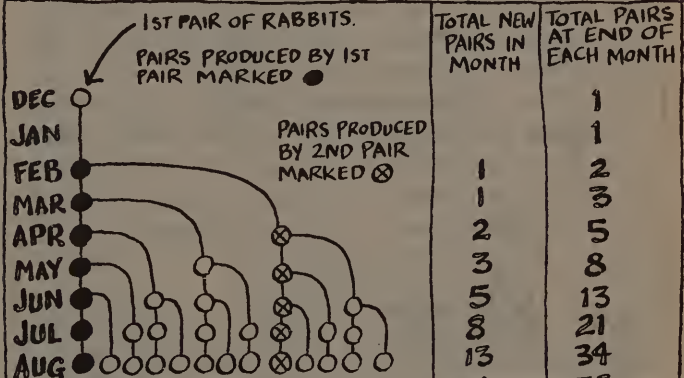
\includegraphics[width=0.75\linewidth]{Photos/Rabbits fibbonacci.png}
    \caption{The rabbit graph, source: Murderous Math: The Key to Universe}
    
\end{figure}
We can notice that the number of pairs of rabbits in a given month follow the sequence are:\\
$1, 1, 2,3, 5, 8, \dots$\\
The pattern is evident. The mathematician's name was Fibonacci and this sequence is called the Fibonacci sequence after him.\\
What happened of the rabbits? They were plentiful in Pisa(couldn't override the town as they neither live or breed for eternity)  and most either lived happily chewing on grass near the white tower. It is believed that their descendants are still there, chewing on the grass, unaware about their contribution.\\
But back to math, a series which depends on its previous terms for its further terms is called a recursive series. We studied about them from a combinatorial perspective in chapter 7. Most of it still applies, and I recommend that you go through it if you haven't already.\\
\begin{xcb}{Exercises}
\begin{enumerate}
\item (AIME) Find the eighth term of the sequence $1440, 1716, 1848,\dots$ whose terms are formed by multiplying the corresponding terms of two arithmetic sequences.
\item(AIME) Two geometric sequences $a_1, a_2, a_3, \ldots$ and $b_1, b_2, b_3, \ldots$ have the same common ratio, with $a_1 = 27$, $b_1=99$, and $a_{15}=b_{11}$. Find $a_9$.
\item (AIME) For $-1<r<1$, let $S(r)$ denote the sum of the geometric series\[12+12r+12r^2+12r^3+\cdots .\]Let $a$ between $-1$ and $1$ satisfy $S(a)S(-a)=2016$. Find $S(a)+S(-a)$
\item (AIME) An infinite geometric series has sum 2005. A new series, obtained by squaring each term of the original series, has 10 times the sum of the original series. The common ratio of the original series is $\frac mn$ where $m$ and $n$ are relatively prime integers. Find $m+n.$
\item (AIME) Call a $3$-digit number geometric if it has $3$ distinct digits which, when read from left to right, form a geometric sequence. Find the difference between the largest and smallest geometric numbers.
\item (AIME) The sum of an infinite geometric series is a positive number $S$, and the second term in the series is $1$. What is the smallest possible value of $S?$
\item (AIME) In an increasing sequence of four positive integers, the first three terms form an arithmetic progression, the last three terms form a geometric progression, and the first and fourth terms differ by $30$. Find the sum of the four terms.
\item (AIME) A sequence of positive integers with $a_1=1$ and $a_9+a_{10}=646$ is formed so that the first three terms are in geometric progression, the second, third, and fourth terms are in arithmetic progression, and, in general, for all $n\ge1,$ the terms $a_{2n-1}, a_{2n}, a_{2n+1}$ are in geometric progression, and the terms $a_{2n}, a_{2n+1},$ and $a_{2n+2}$ are in arithmetic progression. Let $a_n$ be the greatest term in this sequence that is less than $1000$. Find $n+a_n.$
\item (AIME) Consider the sequence defined by $a_k =\dfrac{1}{k^2+k}$ for $k\geq 1$. Given that $a_m+a_{m+1}+\cdots+a_{n-1}=\dfrac{1}{29}$, for positive integers $m$ and $n$ with $m<n$, find $m+n$.
\item (AIME) Given that
\begin{align*}x_{1}&=211,\\ x_{2}&=375,\\ x_{3}&=420,\\ x_{4}&=523,\ \text{and}\\ x_{n}&=x_{n-1}-x_{n-2}+x_{n-3}-x_{n-4}\ \text{when}\ n\geq5, \end{align*}
find the value of $x_{531}+x_{753}+x_{975}$.
\item (AIME) The sequence $\{a_n\}$ is defined by\[a_0 = 1,a_1 = 1, \text{ and } a_n = a_{n - 1} + \frac {a_{n - 1}^2}{a_{n - 2}}\text{ for }n\ge2.\]The sequence $\{b_n\}$ is defined by\[b_0 = 1,b_1 = 3, \text{ and } b_n = b_{n - 1} + \frac {b_{n - 1}^2}{b_{n - 2}}\text{ for }n\ge2.\]Find $\frac {b_{32}}{a_{32}}$.
\item (AIME 2004) Consider the sequence defined by $a_k =\dfrac{1}{k^2+k}$ for $k\geq 1$. Given that $a_m+a_{m+1}+\cdots+a_{n-1}=\dfrac{1}{29}$, for positive integers $m$ and $n$ with $m<n$, find $m+n$.
\item (AIME 1989) If the integer $k$ is added to each of the numbers $36, 300,$ and $596$ one obtains
the squares of three consecutive terms of an arithmetic series. Find $k$.
\item Compute this sum:\\
$(\frac{1}{2^2}+\frac{1}{3^2}+\dots)+(\frac{1}{2^3}+\frac{1}{3^3}+\dots)+\dots$
\item (Putnam 2013,edited) For positive integers $n$, let the numbers $c(n)$ be determined by the rules: $c(1) = 1, c(2n) = c(n),$ and $c(2n + 1) = (-1)^nc(n)$. Find the value of:\\
\[\sum_{n=1}^{2023}c(n)c(n+2)\]
\item If $a, b,c$ form an arithmetic progression, and
$a = x^2 + xy + y^2\\
b = x^2 + xz + z^2\\
c = y^2 + yz + z^2$
where $x + y + z = 0$, prove that $x$, $y$, and $z$ also form an arithmetic progression.
\item (IOQM 2023) The sequence $a_n$ with $n\geq 0$ is defined by $a_0 = 1, a_1 = -4$ and $a_{n+2} = -4a_{n+1}- 7a_n$ for $n \geq 0$ . Find $a_{50}^2 - a_{49}a_{51}$
\item \item (AMC 12) \points{5} Three balls are randomly and independently tossed into bins numbered with the positive integers so that for each ball, the probability that it is tossed into bin i is $2^{-i}$ for $i = 1, 2, 3, \dots$. More than one ball is allowed in each bin. The probability that the balls end up evenly spaced in distinct bins is $p/q$ , where p and q are relatively prime positive integers. (For example, the balls are evenly spaced if they are tossed into bins 3, 17, and
10.) What is $p + q$?

\end{enumerate}
\end{xcb}